% Packages (fold)
\RequirePackage{lmodern}
\documentclass[12pt, oneside, extrafontsizes]{memoir}  % TODO 12pt, twoside

\setstocksize{11in}{8.5in}
\settrimmedsize{11in}{8.5in}{*}
\settrims{0in}{0in}
\setlrmarginsandblock{25mm}{25mm}{*}
\setulmarginsandblock{25mm}{25mm}{*}
\setheadfoot{13pt}{26pt}
\setheaderspaces{*}{13pt}{*}
\checkandfixthelayout
\DoubleSpacing
\setsecnumdepth{subsubsection}
\headstyles{default}
\chapterstyle{ell}
\setsecheadstyle{\scshape\LARGE\raggedright}

\usepackage[colorlinks,bookmarksnumbered,bookmarksdepth=subsubsection,unicode=true]{hyperref}
\newsubfloat{figure}  % must follow hyperref
\hypersetup{
pdfauthor = {Matthew Grenander},
pdftitle = {Learning to Balance Lead Bias in News Summarization},
pdfsubject = {Subject},
pdfkeywords = {natural language processing, automatic summarization, deep learning, machine learning},
pdfcreator = {LaTeX with the hyperref package},
pdfproducer = {},
linkcolor = [HTML]{000000},
citecolor = [HTML]{0000FF},
%urlcolor = [HTML]{\colorc}
}
\usepackage{amsmath}
\usepackage{amsfonts}
\usepackage{amssymb}
\usepackage{amsthm}
\usepackage{diagbox}
\usepackage{dsfont}
\usepackage{mathtools}
\usepackage{xspace}
\usepackage{tikz}
\usetikzlibrary{shapes,arrows}
\usepackage{standalone}
\usepackage{color,soul}
\usepackage[boxed]{algorithm2e}

% Custom commands
\newcommand{\rvs}{r.v.'s\xspace}
\newcommand{\mdp}{Markov Decision Process\xspace}
\newcommand{\mdps}{Markov Decision Processes\xspace}
\newcommand{\mrp}{Markov Reward Process\xspace}
\newcommand{\mc}{Markov Chain\xspace}

\def\given{\;\middle\vert\;}
\def\optimal{\star}
\def\transpose{\intercal}
\def\laplacian{\mathbf{\mathcal{L}}}
\def\eqdef{\overset{\underset{\mathrm{def}}{}}{=}}
\def\indicator{\mathds{1}}
\DeclareMathOperator{\expectation}{\mathbb{E}}
\DeclareMathOperator{\vol}{\text{vol}}
\DeclareMathOperator*{\argmax}{\arg\!\max}
\DeclareMathOperator{\KL}{KL}
\DeclareMathOperator{\rougen}{ROUGE-N}
\DeclareMathOperator{\rougeone}{ROUGE-1_{F1}}
\DeclareMathOperator{\rougetwo}{ROUGE-2_{F1}}
\DeclareMathOperator{\rougel}{ROUGE-L_{F1}}
\DeclarePairedDelimiterX{\infdivx}[2]{(}{)}{%
  #1\;\delimsize\|\;#2%
}
\newcommand{\infdiv}{D_{\KL} \infdivx}

\newcommand{\Drandom}{$D_{\mathrm{random}}$}
\newcommand{\Dinorder}{$D_{\mathrm{inorder}}$}
\newcommand{\Dearly}{$D_{\mathrm{early}}$}
\newcommand{\Dlate}{$D_{\mathrm{late}}$}
\newcommand{\Dmedian}{$D_{\mathrm{med}}$}
\newcommand{\Dall}{$D_{\mathrm{all}}$}
\newcommand{\Dtwenty}{$D_{\mathrm{20}}$}
\newcommand{\Dthirty}{$D_{\mathrm{30}}$}
\newcommand{\Dfifty}{$D_{\mathrm{50}}$}
\newcommand{\Dsixty}{$D_{\mathrm{60}}$}
\newcommand{\BanSumEarly}{$\mathrm{BanditSum+BERT_{early}}$}
\newcommand{\BanSumLate}{$\mathrm{BanditSum+BERT_{late}}$}

\newcommand{\todo}[1]{[TODO: #1]}
\newcommand{\termidx}[1]{\index{#1}{\textbf{#1}}}

\theoremstyle{plain}
\newtheorem{thm}{Theorem}[section]
\newtheorem{lem}[thm]{Lemma}
\newtheorem{prop}[thm]{Proposition}
\newtheorem*{cor}{Corollary}

\theoremstyle{definition}
\newtheorem{defn}{Definition}[section]
\newtheorem{conj}{Conjecture}[section]
\newtheorem{exmp}{Example}[section]

\usepackage[utf8]{inputenc}
\usepackage{csquotes}
\usepackage{showidx}
\makeindex

\usepackage[backend=biber, citestyle=authoryear, bibstyle=authoryear, isbn=false, url=false, doi=false, eprint=false, natbib=false, sorting=nty, uniquename=init]{biblatex}
\addbibresource{library.bib}

\begin{document}

%%%%%%%%%%%%%%%%%%%%%%%%%%%%%%%%%%%%%%%%%%%%%%%%%%%%%
% Title page
%%%%%%%%%%%%%%%%%%%%%%%%%%%%%%%%%%%%%%%%%%%%%%%%%%%%%

% Title (fold)
\pretitle{\begin{center}\cftchapterfont\huge}
\posttitle{\end{center}}
\preauthor{\begin{center}\huge}
\postauthor{\end{center}}
\predate{\begin{center}\large}
\postdate{\end{center}}

\title{Learning to Balance Lead Bias in News Summarization}
\author{Matt Grenander}
\date{\today}
\renewcommand\maketitlehookb{
\vfill
}
\renewcommand\maketitlehookc{
\vfill
\begin{center}
{
\large
Department of Computer Science\\
McGill University, Montreal
}
\end{center}
\vspace{10mm}
}
\renewcommand\maketitlehookd{
\vspace{10mm}
\begin{center}
A thesis submitted to McGill University in partial fulfilment of the requirements of
the degree of Master of Science. \\
\copyright 2020 Matt Grenander
\end{center}
}
% Title (end)

\begin{titlingpage}
\maketitle
\end{titlingpage}

%%%%%%%%%%%%%%%%%%%%%%%%%%%%%%%%%%%%%%%%%%%%%%%%%%%%%
% Ackowledgements
%%%%%%%%%%%%%%%%%%%%%%%%%%%%%%%%%%%%%%%%%%%%%%%%%%%%%
%\clearpage
%\pagenumbering{roman}
%\renewcommand{\abstractname}{Dedication}

%%%%%%%%%%%%%%%%%%%%%%%%%%%%%%%%%%%%%%%%%%%%%%%%%%%%%
% Ackowledgements
%%%%%%%%%%%%%%%%%%%%%%%%%%%%%%%%%%%%%%%%%%%%%%%%%%%%%
\clearpage
\pagenumbering{roman}
\renewcommand{\abstractname}{Acknowledgements}
\begin{abstract}
% Annie and Jackie
First, I would like to thank my supervisors Jackie Chi Kit Cheung and Annie Louis. I am thankful for their guidance in exploring research topics, carrying out practical research and communicating these ideas effectively. They have helped me think critically and become a better researcher.

% Friends and colleagues
I also want to thank my colleagues and friends at MILA for their helpful discussions, patience and feedback. In particular, I am grateful to Yue Dong for our many conversations that led to new research directions and collaborations.
\end{abstract}

%%%%%%%%%%%%%%%%%%%%%%%%%%%%%%%%%%%%%%%%%%%%%%%%%%%%%
% Abstract
%%%%%%%%%%%%%%%%%%%%%%%%%%%%%%%%%%%%%%%%%%%%%%%%%%%%%
\clearpage
\renewcommand{\abstractname}{Abstract}
\begin{abstract}
As technology increases the tremendous amount of text we encounter each day, a clear need has arisen for tools to filter out noise and highlight key phrases.
\textbf{Automatic summarization} systems have emerged as a viable solution to sort through and intelligently condense text.
In this thesis, we focus on \textbf{extractive summarization}, in which the system selects text snippets from a source document that best represent the given text.
Extractive summarization systems must learn complex lexical representations so that they are able to rank sentences in order of relevance, while minimizing redundancy in the output summary.
For news articles, extractive summarization systems have been shown to exhibit a bias towards selecting content from an article's lead sentences, even when these sentences are irrelevant to the overall text \parencite{kedzie2018content}.
We investigate this phenomenon in detail, showing that when an article's sentence order is permuted, state-of-the-art systems drastically underperform.
To alleviate this problem, we propose an auxiliary objective function which encourages the model to look beyond a document's leading sentences and properly value each sentence.
We show that this auxiliary objective significantly improves summarization performance, particularly in cases where the article's leading sentences constitute a poor summary.
We extend this approach to a novel summarization method that classifies documents into two distinct groups: ones in which leading phrases constitute a strong summary, and ones in which they form a poor sumary. Two separate systems then summarize the two groups.
We show that this approach is promising, though more work is needed towards accurately classifying articles.
\end{abstract}

\clearpage
\renewcommand{\abstractname}{Abrégé}
\begin{abstract}
L’usage de la technologie au quotidien nous confrontant à de plus en plus à d’éléments textuels, nous avons plus que jamais besoin d’outils pour filtrer et synthétiser les concepts clés dans un corps de texte.
Les \textbf{systèmes de résumé automatiques} apparaissent comme des solutions viables pour organiser et condenser du texte intelligemment. 
Dans cette thèse, nous nous concentrons sur \textbf{la synthèse extractive}, dans laquelle le système sélectionne les extraits du document source représentant au mieux l’idée générale du texte.
Les systèmes extractifs doivent apprendre des représentations lexicales complexes afin de pouvoir classer les phrases par ordre de pertinence, tout en minimisant leur redondance dans le résumé final. 
Pour les articles de presse, il a été démontré que les systèmes extractifs présentent un biais car ils sélectionnent d’emblée les premières phrases de l’article, même lorsque ces phrases ne sont pas pertinentes pour résumer le texte global \parencite{kedzie2018content}.
Nous étudions ce phénomène en détail, en démontrant le déclin drastique des performances de technologies de pointe lorsque l’ordre des phrases au sein d’un article est perturbé.
Pour atténuer ce problème, nous proposons un objectif auxiliaire qui encourage le modèle à poursuivre son analyse au-delà des premières phrases d'un document, et à évaluer correctement chaque phrase. 
Nous montrons que cet objectif auxiliaire améliore considérablement la qualité de synthèse, en particulier dans les cas où les premières phrases de l'article constituent un mauvais résumé. 
Nous étendons cette approche à une nouvelle méthode de synthèse, qui classe les documents en deux groupes distincts : ceux dont les premières phrases constituent un bon résumé, et ceux pour lesquelles elles sont insuffisantes. Des systèmes séparés résument les deux groupes.
Nous montrons que cette approche est prometteuse, bien qu’il soit nécessaire d’optimiser davantage le système pour classer les articles avec plus de précision.
\end{abstract}

%%%%%%%%%%%%%%%%%%%%%%%%%%%%%%%%%%%%%%%%%%%%%%%%%%%%%
% Table of content
%%%%%%%%%%%%%%%%%%%%%%%%%%%%%%%%%%%%%%%%%%%%%%%%%%%%%
\clearpage
\setcounter{tocdepth}{2}
\tableofcontents
\newpage
\listoffigures
\newpage
\listoftables

%%%%%%%%%%%%%%%%%%%%%%%%%%%%%%%%%%%%%%%%%%%%%%%%%%%%%
% Introduction
%%%%%%%%%%%%%%%%%%%%%%%%%%%%%%%%%%%%%%%%%%%%%%%%%%%%%
\clearpage
\pagenumbering{arabic}
\chapter{Introduction}
Extractive summarization remains a simple 
and fast approach to produce summaries which 
are grammatical and accurately represent the source text.
In the news domain, these systems are able to 
use a dominant signal: the position of a sentence 
in the source document. 
Due to journalistic conventions which place important information
early in the articles, the lead sentences often contain key information. In this paper, we explore how systems can look beyond this simple trend. 

Naturally, automatic systems have 
all along exploited position cues in news 
as key indicators of important content \parencite{schiffman,hong2014improving,ext_bert}. 
The `lead' baseline is rather strong in single-document news summarization \parencite{brandow1995automatic,nenkova2005automatic}, 
with automatic systems only modestly improving the results. 
Nevertheless, more than 20-30\% of 
summary-worthy sentences come from the second half of news documents \parencite{data2_nallapati2016abstractive,kedzie2018content}, 
and the lead baseline, as shown in Table \ref{tab:lead_ex},
does not always produce convincing summaries.
So, systems must balance the position bias with representations of the semantic content 
throughout the document. Alas, preliminary studies
\parencite{kedzie2018content} suggest that even the most recent neural 
methods predominantly pick sentences from the lead, and 
that their content selection performance drops greatly
when the position cues are withheld.

\begin{table}[t]
    \centering
    \small
    \begin{tabular}{|p{0.94\linewidth}|}
        \hline
        \textbf{Lead-3:} Bangladesh beat fellow World Cup quarter-finalists Pakistan by 79 runs in the first one-day international in Dhaka. Tamim Iqbal and Mushfiqur Rahim scored centuries as Bangladesh made 329 for six and Pakistan could only muster 250 in reply. Pakistan will have the chance to level the three-match series on Sunday when the second odi takes place in Mirpur. \\ \hline
        \textbf{Reference:} Bangladesh beat fellow World Cup quarter-finalists Pakistan by 79 runs. Tamim Iqbal and Mushfiqur Rahim scored centuries for Bangladesh. Bangladesh made 329 for six and Pakistan could only muster 250 in reply. Pakistan will have the chance to level the three-match series on Sunday. \\ \hline \hline
        \textbf{Lead-3}: Standing up for what you believe. What does it cost you? What do you gain? \\ \hline
        \textbf{Reference:} Indiana town's Memories Pizza is shut down after online threat. Its owners say they'd refuse to cater a same-sex couple's wedding. \\
        \hline
    \end{tabular}
    \caption{`Lead' (first 3 sentences of source) can produce extremely faithful (top) to disastrously inaccurate (bottom) summaries. Gold standard summaries are also shown.}
    \label{tab:lead_ex}
\end{table}

In this paper, we verify that 
sentence position and lead bias dominate the 
learning signal for  state-of-the-art neural 
extractive summarizers in the news domain. 
We then present techniques to improve content selection in 
the face of this bias. 
The first technique makes use of `unbiased data' 
created by permuting the order of sentences in the training
articles. We use this shuffled dataset for pre-training, followed by 
training on the original (unshuffled) articles. 
The second method introduces an auxiliary loss 
which encourages the model's scores for sentences 
to mimic an estimated score distribution over the
sentences, the latter computed using ROUGE overlap 
with the gold standard. We implement these techniques 
for two recent reinforcement learning based systems, 
RNES \parencite{DBLP:conf/aaai/WuH18} and 
BanditSum \parencite{dong2018banditsum}, and evaluate 
them on the CNN/Daily Mail dataset \parencite{hermann2015teaching}.

We find that our auxiliary loss achieves 
significantly better ROUGE scores
compared to the base systems, and that the 
improvement is even more pronounced when the true 
best sentences appear later in the article. 
On the other hand, the pretraining approach produces mixed results.
We also confirm that when summary-worthy sentences 
appear late, there is a large performance discrepancy 
between the oracle summary and state-of-the-art summarizers,
indicating that learning to balance lead bias with 
other features of news text is a noteworthy issue to tackle.

\subsection{Outline}

Basic theory of stochastic processes and Markov chains is first presented in chapter \ref{chap:decisionmaking}. The inclusion of this material is motivated by the probabilistic interpretation of spectral graph theory studied in chapter \ref{chap:dynamics}. The theory of Markov Decision Processes is presented in section \ref{sec:mdp} as a necessary prerequisite for the appreciation of the techniques developed in reinforcement learning. Chapter \ref{chap:temporalabstraction} focuses on the presentation of the options framework \parencite{Sutton1999} in reinforcement learning as a way to represent temporal abstraction and learn optimal control over it.

The connection from graph \textit{structure} to system \textit{dynamics} is developed throughout chapter \ref{chap:dynamics} and is instrumental is understanding the strengths and pitfalls of the graph partitioning approach for options discovery. It also allows a better understanding of the relevant work on Nearly-Completely Decomposable Markov Chains (NCD) for future theoretical research on the bottleneck concept. The NCD theory seems to call for an information theoretic comprehension of temporal abstraction which is briefly developed at the end of this section.

A new algorithm for options discovery is proposed in chapter \ref{chap:buildingoptions} based on the  \textsc{Walktrap} community detection algorithm of \cite{Pons2005}. Although \textsc{Walktrap} finds its roots into spectral graph theory, its running time is only order $\mathcal{O}(mn^2)$ rather than $\mathcal{O}(n^3)$ by avoiding to compute the eigenvectors explicitly. The problem of options discovery and construction is also set under the assumption of a continuous state space. Techniques for constructing proximity graphs in Euclidean space are developed in section \ref{sec:proximitygraphs}. Section \ref{sec:knnoptions} shows how approximate nearest neighbors algorithms can be used to properly define the initiation and termination components of options under continuous observations.

An illustration of the proposed algorithm is provided in chapter \ref{chap:illustration} with the Pinball domain of \cite{Konidaris2009}. Practical difficulties having to do oscillations and off-policy learning are analysed. The proper empirical choices for the number of nearest neighbors, type of proximity graph and time scale for the \textsc{Walktrap} algorithm are discussed.

%%%%%%%%%%%%%%%%%%%%%%%%%%%%%%%%%%%%%%%%%%%%%%%%%%%%%
% Background / Related Work
%%%%%%%%%%%%%%%%%%%%%%%%%%%%%%%%%%%%%%%%%%%%%%%%%%%%%
\chapter{Background}
\label{chap:relatedwork}

Modern summarization methods for news are typically
based on neural network-based sequence-to-sequence learning
\parencite{cnn1_kalchbrenner2014convolutional,cnn2_kim2014convolutional,rnn2_chung2014gru,ext2_2015Yin,ext3_cao2015learning,ext4_cheng2016neural,ext5_summarunner,narayan2018don,neusum}.
In MLE-based training, extractive summarizers are 
trained with gradient ascent to maximize the likelihood
of heuristically-generated ground-truth binary
labels \parencite{ext5_summarunner}. Many MLE-based models
do not perform as well as their reinforcement 
learning-based (RL) competitors that directly optimize ROUGE \parencite{abs5_paulus2017deep,DBLP:Narayan/2018,dong2018banditsum,DBLP:conf/aaai/WuH18}. 
As RL-based models represent the state of the art for 
extractive summarization, we analyze them in this paper.

The closest work to ours is a recent study by 
\cite{kedzie2018content} which showed that 
MLE-based models learn a significant bias for 
selecting early sentences when trained on news 
articles as opposed to other domains. As much as 
58\% of selected summary sentences come directly 
from the lead. Moreover, when these models
are trained on articles whose sentences
are randomly shuffled, the performance drops 
considerably for news domain only. While this drop 
could be due to the destruction of position cues, 
it may also arise because the article's coherence
and context were lost. 

In this paper, we employ finer control on the 
distortion of sentence position, coherence, and 
context, and confirm that performance drops are 
mainly due to the lack of position cues. 
We also propose the first techniques to 
counter the effects of lead bias in neural extractive systems.


%%%%%%%%%%%%%%%%%%%%%%%%%%%%%%%%%%%%%%%%%%%%%%%%%%%%%
% Perturbing Sentence Order
%%%%%%%%%%%%%%%%%%%%%%%%%%%%%%%%%%%%%%%%%%%%%%%%%%%%%
% \chapter{Perturbing Sentence Order}
% \label{chap:perturb}
% \input{chapters/perturb}

%%%%%%%%%%%%%%%%%%%%%%%%%%%%%%%%%%%%%%%%%%%%%%%%%%%%%
% Countering Lead Bias via Auxiliary Loss
%%%%%%%%%%%%%%%%%%%%%%%%%%%%%%%%%%%%%%%%%%%%%%%%%%%%%
\chapter{Countering Lead Bias via Auxiliary Loss}
\label{chap:aux_loss}
% Intro
A recent study by \cite{kedzie2018content} shows that MLE-based summarization models learn a significant bias towards selecting early sentences when trained on news articles, a phenomenon they term `lead bias'. They demonstrate that in some models, as much as 58\% of selected summary sentences come directly from the article's leading sentences. Moreover, when these models are trained on news articles whose sentences are randomly shuffled, the performance drops considerably on the news domain.

These results suggest that lead bias is a significant bottleneck for news summarization systems. For this reason, we would like to explore the severity of this issue further and design potential solutions. In this chapter, we corroborate and expand on \cite{kedzie2018content}'s findings by perturbing sentence order in news articles in a multitude of ways. These experiments confirm that positional cues dominate the learning signals for state-of-the-art summarization systems.

We then detail our method for countering lead bias, based around augmenting an existing summarization system with an auxiliary loss objective aimed at properly evaluating sentence relevance independent of sentence position. We demonstrate that this method is able to decrease the percentage of time the base model selects leading sentences, while also improving the model's overall summary quality. The resulting model is particularly more adept at summarizing articles where the lead performance is weak, indicating that our method is effective at helping models look beyond simple positional cues.

\section{Base model: BanditSum}
% Intro paragraph: why BanditSum?
In order to experiment with lead bias in modern summarization models, we first need to choose a model to analyze. Here, we detail BanditSum's formulation, and why it lends itself well to lead bias experiments.

% Brief overview of how BanditSum works
BanditSum approaches extractive summarization as a contextual bandit problem. This approach views the document as a context, while selecting a subset of sentence indices corresponds to an action. Sentences are first mapped to \textit{sentence affinity} scores, representing the model's propensity to include each sentence in its summary. The authors then take advantage of reinforcement learning techniques, interpreting these affinity scores as a stochastic policy. BanditSum uses the REINFORCE algorithm \parencite{williams1992simple} to compute policy gradient updates, avoiding the MLE-based summarization issues raised by \cite{DBLP:Narayan/2018}. The authors also confirm empirically that BanditSum's non-autoregressive framework enables it to sidestep some lead bias issues faced by other autoregressive summarization systems.

\subsection{Model Architecture}
\begin{figure}[h]
    \centering
    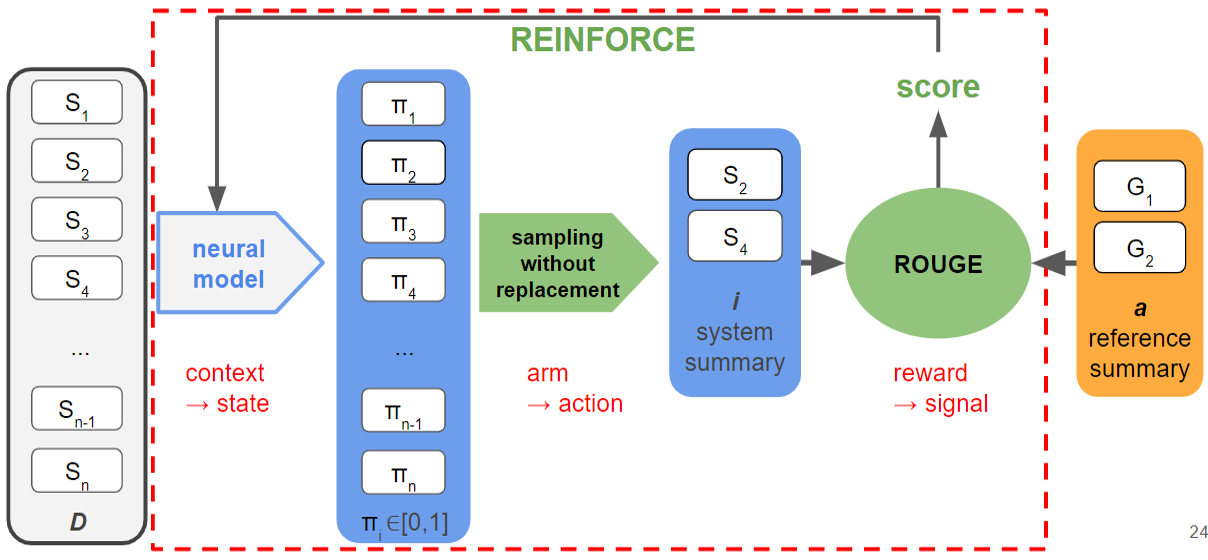
\includegraphics[width=0.9\linewidth]{fig/bsum_architecture.png}
    \caption[An overview of the BanditSum model.]{An overview of the BanditSum model. Sentence affinity scores are sampled to create hypothesis summaries, which are then scored against a reference summary using ROUGE. A gradient update is then computed using REINFORCE. Figure created by Yue Dong and used with permission.}
    \label{fig:bsum_architecture}
\end{figure}

Given a document $D$ with $n$ sentences, the neural model produces sentence affinity scores $\pi_\theta = \{ \pi_1,\dots,\pi_n \}$, where $\pi_i \in [0, 1]$.
After first using GloVe \parencite{we2_pennington2014glove} to embed each word, a word-level LSTM captures interword dependencies. In each sentence, these word representations are averaged and then passed to a sentence-level LSTM to create sentence features $h_1,\dots,h_n$. Finally, a multi-layer perceptron decoder maps $h_1,\dots,h_n$ to the sentence affinity scores $\pi_\theta = \{\pi_1,\dots,\pi_n \}$.

% Reinforcement Learning-based Objective
Using the sentence affinity scores, BanditSum now computes a gradient update following the REINFORCE algorithm \parencite{williams1992simple}. In particular, hypothesis summaries are repeatedly sampled according to $\pi_\theta$, consisting of $K$ sentences each\footnote{The authors use $K = 3$ following the average reference summary sentence length.}. Each hypothesis summary is then scored against the reference summary using a reward function based on ROUGE:

\begin{equation}
    \mathrm{R}(\mathcal{S}, \mathcal{R}_D) = \frac{1}{3}\left( \rougeone(\mathcal{S}, \mathcal{R}_D) + \rougetwo(\mathcal{S}, \mathcal{R}_D) + \rougel(\mathcal{S}, \mathcal{R}_D) \right)
\end{equation}

where $\mathcal{S}$ is the system summary and $\mathcal{R}_D$ is the reference summary. Finally, using a self-critical baseline $\overline{r}$ for variance reduction \parencite{rennie2017self}, they compute the policy gradient update as follows:

\begin{equation}
    \nabla_\theta J(\theta) = \frac{1}{B} \sum_{i=1}^{B} \nabla_\theta \log p_\theta(\mathcal{S}_i \vert D)  \left[\mathrm{R}(\mathcal{S}_i, \mathcal{R}_D) - \overline{r} \right] 
\end{equation}

where $p_\theta (\mathcal{S}_i \vert D)$ is the joint probability of including the sentences in $\mathcal{S}_i$ (i.e. according to $\pi_\theta$). This equation corresponds to the update equation given by REINFORCE \cite{williams1992simple}.

\subsection{Analysis}
% D_early vs D_late experiments, non-autoregressivity
One of BanditSum's key properties is that the model is \textbf{non-autoregressive}, meaning that the decision to include sentence $s_i$ does not explicitly depend on sentences $s_1,\dots,s_{i-1}$. An example of an autoregressive model is given by SummaRuNNer \parencite{ext5_summarunner}, whose ``summary-so-far'' representation recursively depends on previous summary decisions (see Equations \ref{eq:autoregressive-1} and \ref{eq:autoregressive-2}).

\begin{figure}[t]
    \centering
    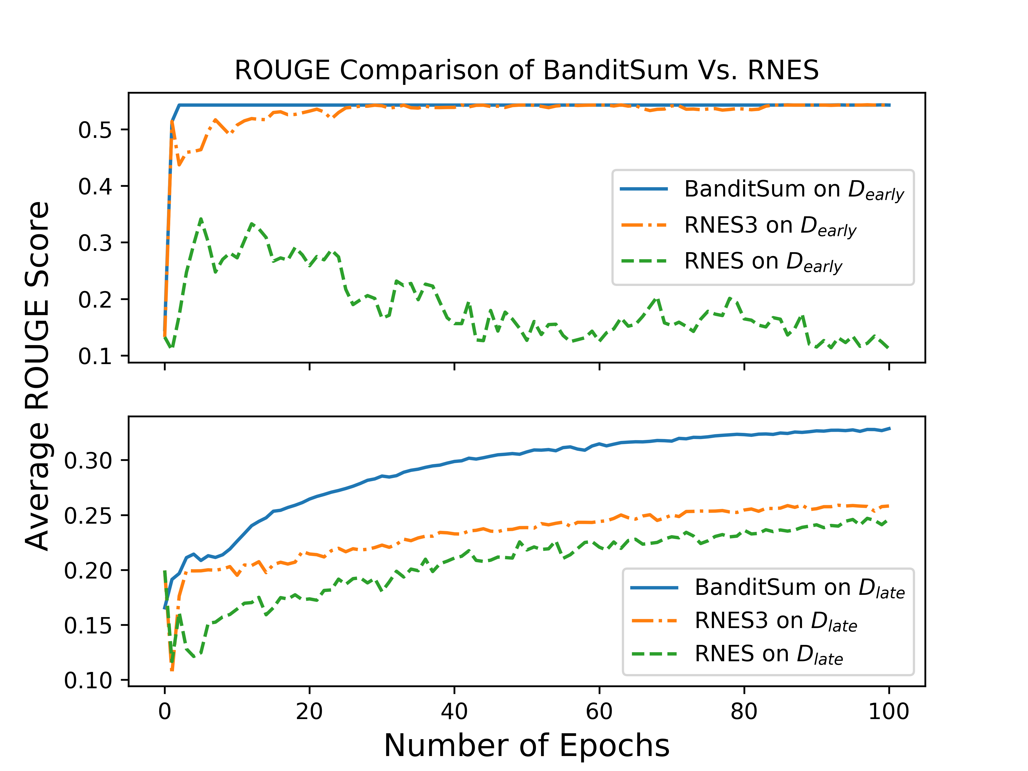
\includegraphics[width=0.8\linewidth]{fig/bsum_early_late.png}
    \caption[Comparison of BanditSum and RNES on \Dearly{} and \Dlate{} subsets.]{Comparison of BanditSum and RNES on \Dearly{} and \Dlate{} subsets. While performance is roughly similar on \Dearly{}, BanditSum dominates over RNES on \Dlate{}. Figure from \cite{dong2018banditsum}.}
    \label{fig:bsum_early_late}
\end{figure}

BanditSum's authors conjecture that autoregressive models are more likely to suffer from lead bias issues. Autoregressive models must decide whether to include early sentences before fully evaluating later sentences, and this may lead the models to erroneously include earlier sentences in their summaries. To verify this claim, the authors annotate articles from the validation set by an extractive index $\overline{idx}$, denoting whether an oracle-generated extractive summary appears earlier or later in the document. Articles are then sorted according to  $\overline{idx}$, and two datasets are created. \Dearly{} is formed from the top 50 documents w.r.t. $\overline{idx}$ (i.e. best summary appears earlier), while \Dlate{} contains the lowest-scoring 50 articles (i.e. best summary appears late). Finally, both BanditSum and an autoregressive model RNES \parencite{DBLP:conf/aaai/WuH18} are trained and evaluated on the \Dearly{} and \Dlate{} subsets. The results are displayed in Figure \ref{fig:bsum_early_late}.

% Results from this experiment
While BanditSum and RNES perform similarly on \Dearly{}, BanditSum eclipses RNES on \Dlate{}, converging much quicker to higher scoring summaries. Owing to its non-autoregressive formulation, BanditSum can produce more effective summaries when summary-worthy sentences occur later in the article. This fact provides a good basis for performing lead bias experiments with BanditSum, as we would prefer a model that is not inherently biased towards earlier occurring sentences.

\section{Lead Bias of News Systems}\label{sec:perturb}
While the observed performance drops in \cite{kedzie2018content} may be due to the destruction of position cues, they may also arise because the article's coherence and context were lost. We explore this phenomenon more deeply by distorting sentence order in a multitude of ways. 

We manipulate the CNN / Daily Mail dataset to preserve sentence position information at different levels. For each setting, we train separate instances of BanditSum, then test the model on the other datasets. In the \textbf{random} setting, sentences are shuffled randomly; in \textbf{reverse}, they are in reverse order; in \textbf{insert-lead} and \textbf{insert-lead3}, we insert an out-of-document sentence (chosen randomly from the corpus) as the first sentence or randomly as one of the first three sentences, respectively. Finally, \textbf{original} preserves the original ordering.

\begin{table}[t]
\centering
\small
\begin{tabular}{c|ccccc}
\toprule
\diagbox{Train setting}{Test setting}	&	original	&	random	&	reverse	&	insert-lead	&	insert-lead3	\\ \hline
Lead-3 baseline	&	32.68	&	22.81	&	17.94	&	27.67	&	27.68	\\ \hline
original	&	\textbf{33.85}	&	26.18	&	20.71	&	31.71	&	31.11	\\
random	&	30.88	&	\textbf{29.70}	&	29.79	&	29.97	&	30.09	\\
reverse	&	21.35	&	26.32	&	\textbf{33.59}	&	21.63	&	21.65	\\
insert-lead	&	33.21	&	26.07	&	20.70	&	\textbf{33.41}	&	31.59	\\
insert-lead3	&	32.29	&	25.57	&	20.22	&	32.92	&	\textbf{32.15}	\\ \bottomrule
\end{tabular}
\caption[BanditSum's performance on perturbed datasets]{BanditSum's performance---calculated as the average between ROUGE-1,-2, and -L F1---on the CNN/Daily Mail validation set. The sentence position information is perturbed at different levels.}
\label{tab:data_manipulation}
\end{table}

\begin{table}[t]
    \centering
    \begin{tabular}{c|c|c}
    \toprule
    Train setting	&	Average of ROUGE-1, -2, -L	&	Standard Deviation	\\ \hline
    Lead-3 baseline	&	25.76	&	5.00	\\ \hline
    original	&	28.71	&	4.72	\\
    random	&	\textbf{30.09}	&	\textbf{0.42}	\\
    reverse	&	24.91	&	4.72	\\
    insert-lead	&	29.00	&	4.93	\\
    insert-lead3	&	28.63	&	4.98	\\ \bottomrule
    \end{tabular}
    \caption[BanditSum's average performance on perturbed datasets.]{Average ROUGE-1, -2 and -L scores and standard deviation on the CNN / Daily Mail validation set using different training settings.}
    \label{tab:data_manipulation_mean}
\end{table}

In Table \ref{tab:data_manipulation} and \ref{tab:data_manipulation_mean}, we show BanditSum's performance when trained and tested on the various datasets.
All models (except random) perform worse when tested on a mismatched data perturbation. Even when the distortion is at a single lead position in \textbf{insert-lead} and \textbf{insert-lead3}, the performance on the original data is significantly lower than when trained without the distortion.

These results corroborate \cite{kedzie2018content}'s findings for RL-based systems. Similar results hold two other models we test: RNES \parencite{DBLP:conf/aaai/WuH18} drops 4.2 and Refresh \parencite{DBLP:Narayan/2018} drops 3.4 points in average ROUGE when trained on shuffled data and tested on the original dataset.

% Conclusions
The results in Table \ref{tab:data_manipulation} are worrying as the large drops between mismatched train and test settings suggest that position cues are a dominating signal for BanditSum. These findings suggest that BanditSum may largely ignore semantic content in favour of cheap positional cues. Obviously, this exploit will not work for news articles where summary-worthy content appears later. Beyond the news domain, other summarization domains may contain their own positional biases and similarly influence automatic learners. More generally, future summarization systems which attempt to create summaries across many domains cannot solely rely on positional cues if these signals change across domains. In order to be effective, systems must learn to balance between exploiting positional cues in the data and understanding the underlying semantic content.

Interestingly, the \textbf{random} model has the 
best mean performance and the lowest variation, indicating that removing or lessening position bias may allow a model to focus on learning robust sentence semantics. Following this observation, we explore novel techniques aimed at reducing the influence of lead bias on the learning process.

\section{Auxiliary Loss Objective}
Motivated by the experiments in Section \ref{sec:perturb}, we set towards designing methods to reduce models' dependence on positional cues. We observe that in general, BanditSum tends to converge to a low-entropy policy, in the sense that the model's affinity scores are either 1 or 0 at the end of training. Regularizing low-entropy policies can increase a model's propensity to explore potentially good states or stay close to a known good policy \parencite{nachum2017improving, galashov2019information}. We extend this idea to summarization by introducing a ROUGE-based loss which regularizes the model policy using an estimate of the value of individual sentences.

As the goal is to guide the model towards properly valuing sentences, we must first approximate the true value of each sentence in a document. These sentence-level estimates are computed as a categorical distribution $P_R$ over the document:
\begin{equation}
    P_R( x = i ) = \frac{r(s_i, \mathcal{G})}{\sum_{j=1}^{n}{r(s_j, \mathcal{G})}}
\end{equation}
where $r$ is the average of ROUGE-1, -2 and -L F\textsubscript{1} scores between sentence $s_i$ in the article and the reference summary $\mathcal{G}$. Since ROUGE measures lexical overlap, this distribution provides a good approximation of each sentence's relevance to the reference answer.

We would like the model's predictive distribution $P_\mathcal{M}$ to approximately match $P_R$. To compute $P_\mathcal{M}$, we normalize the model's predicted sentence scores. In other words, if the model outputs sentence affinity scores $\pi_\theta = (\pi_1,\dots,\pi_n)$, $P_\mathcal{M}$ is computed as:
\begin{equation}
    P_\mathcal{M}(x = i) = \frac{\pi_i}{\sum_{j=1}^n \pi_j}
\end{equation}

Our auxiliary loss is defined as the KL divergence: $\mathcal{L}_{\KL} = \infdiv{P_R}{P_\mathcal{M}}$. We modify the update rule using a weighted sum of the original model loss and our KL-based loss:
\begin{equation}
\label{eq:kl_loss}
    \theta^{(t+1)} = \theta^{(t)} + \alpha \left( \nabla \mathcal{L}_{\mathcal{M}}(\theta^{(t)}) + \beta \nabla \mathcal{L}_{\KL}(\theta^{(t)}) \right)
\end{equation}
Here, $\theta^{(t)}$ represents the model's parameters at time step $t$, $\mathcal{L}_{\mathcal{M}}$ is the original model's loss function, $\alpha$ is the learning rate, and $\beta$ is a hyperparameter.

Notably, $\mathcal{L}_{\KL}$ does not account for redundancy, and we do not use this measure as the sole objective function. In fact, experiments we conduct show that solely using the KL objective function does not result in improved performance.

\section{Experimental Setup}
We test our method using the CNN/Daily Mail dataset \parencite{hermann2015teaching}, building on top of the author-provided BanditSum implementation. To reduce training time, we pre-compute and store the ROUGE-1, -2, and -L average for every sentence triplet of each article, using PyTables and HDF5 \parencite{pytables, hdf5}. This allows for a considerable increase in training speed. We limit the maximum number of sentences considered in an article to the first 100. All the models were trained for 4 epochs. We set the auxiliary loss hyperparameters $\alpha=1e-4$ and $\beta=0.0095$ in Equation \ref{eq:kl_loss} based on a grid search using the Tune library \parencite{tune}.

We also train a baseline entropy model by replacing $\mathcal{L}_{\KL}$ with the negated entropy of $P_\mathcal{M}$ in Equation \ref{eq:kl_loss}. This loss penalizes low entropy, helping the model explore, but it is `undirected' compared to our proposed method. In contrast, the $\mathcal{L}_{\KL}$ loss provides an indication of each sentence's value, and is `directed' in this sense. We present the results of Lead-3 baseline (first 3 sentences), and two other competitive models -- Refresh and NeuSum \parencite{DBLP:Narayan/2018, neusum}. Lastly, we include results from an oracle summarizer, computed as the triplet of source sentences with the highest average of ROUGE-1, -2 and -L scores against the abstractive gold standard.

\section{Results}
\label{sec:result}
\begin{table}[t]
    \centering
    \small
    \begin{tabular}{l|ccc|c}
        \toprule						
        Model	&	\multicolumn{3}{c}{ROUGE}	& Lead Overlap	\\
        	&	1	&	2	&	L	&	\%	\\ \hline
        Lead-3	&	40.06	&	17.53	&	36.18	&   100.0	\\
        Oracle	&	56.53	&	32.65	&	53.12	&	27.24	\\
        Refresh	&	40.0	&	18.2	&	36.6	&	--	\\
        NeuSum	&	40.15	&	17.80	&	36.63	&	58.24	\\
        RNES	&	41.15	&	18.81	&	37.75	&	68.44	\\\hline 
        BanditSum	    &	41.68	&	18.78	&	38.00	&	69.87	\\
        B.Sum+pretrain  &   41.68   &   18.79   &   37.99   &   70.77   \\
        B.Sum+entropy	&	41.71	&	18.87	&	38.04	&	64.83	\\
        BanditSum+KL	&	\textbf{41.81*}	&	\textbf{18.96*}	&	\textbf{38.16*}	&	65.13	\\
        \bottomrule
    \end{tabular}
    \caption[Main results from auxiliary loss method on the CNN / Dailymail dataset.]{ROUGE scores for systems. Lead overlap denotes the model's overlap in extraction choices with the lead-3 baseline. Scores significantly higher than BanditSum with $p<0.001$ (bootstrap resampling test) are marked with *. Note that we are unable to evaluate Refresh on the lead overlap measure due to lack of access to the model outputs.}
    \label{tab:results}
\end{table}

Table \ref{tab:results} reports the F1 scores for ROUGE-1,-2 and -L \parencite{eva1_lin:2004:ACLsummarization}. We use the pyrouge\footnote{\url{www.github.com/bheinzerling/pyrouge}} wrapper library to evaluate the final models, while training with a faster Python-only implementation\footnote{\url{www.github.com/Diego999/py-rouge}}. We test for significance between the baseline models and our proposed techniques using the bootstrap method. This method was first recommended for testing significance in ROUGE scores in the original ROUGE paper \parencite{eva1_lin:2004:ACLsummarization}, and has subsequently been advocated as an appropriate measure in works such as \cite{dror-hitchhikers} and \cite{berg-kirkpatrick}.

The simple entropy regularizer has a small but insignificant improvement, indicating that while boosting exploration is helpful, it is too simple to provide real performance gains. In contrast, the BanditSum+KL method significantly improves over BanditSum, with an extra 0.15 ROUGE points on average. The last column reports the percentage of summary sentences which overlap with the lead. The auxiliary loss leads to a 4.7\% absolute decrease in such selections compared to the base system, while also reaching a better ROUGE score. Figure \ref{fig:train_curves} shows that the reward for the auxiliary loss model is consistently above the base.

\begin{figure}
    \centering
    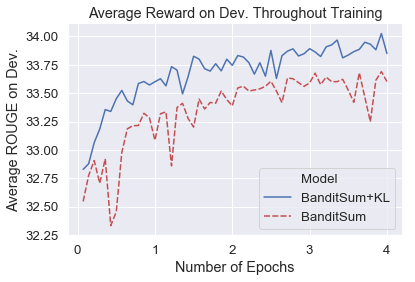
\includegraphics[width=0.75\linewidth]{fig/final_dev_fig.png}
    \caption[Training curves for BanditSum-based models.]{Training curves for BanditSum-based models. Average ROUGE is the average of ROUGE-1, -2 and -L F1.}
    \label{fig:train_curves}
\end{figure}

\section{Analysis}
Given that our method is designed to alleviate overfitting to positional cues, we suspect that the BanditSum+KL model achieves greater gains when the lead constitutes a poor summary. To test this idea, we examine the auxiliary loss model on documents where the summary is mostly comprised of lead sentences \Dearly{}, mostly sentences much later in the article \Dlate{}, and a dataset at the midway point, \Dmedian{}. To create these sets, we compute an extractive index $\overline{idx}$ for each test set document, similar to \cite{dong2018banditsum}. Given a document, we use the oracle summarizer's extracted indices $(i, j, k)$ and compute $\overline{idx}$ as:
\begin{equation}
    \overline{idx} = \frac{i + j + k}{3n}
\end{equation}
where $n$ is the number of sentences in the document.

After the test articles are ranked using the $\overline{idx}$ metric, the 100 test articles with lowest average index are \Dearly{}, the 100 with highest value are \Dlate{} and the 100 closest to the median are \Dmedian{}. In Table \ref{d_early}, we can see that the auxiliary loss model's improvements are even more amplified on \Dmedian{} and \Dlate{}. 

The second line in Table \ref{d_early} reports the oracle ROUGE scores of the best possible extractive summary. While all systems are quite close to the oracle on \Dearly{} they only reach half the performance on \Dlate{}. This gap indicates that our improvements only scratch the surface, but also that this problem is worthy and challenging to explore. 

In Figure \ref{fig:avg_pos}, we compare BanditSum and BanditSum+KL's average affinity scores. The BanditSum+KL method sharply reduces the average affinity score on the first two sentence positions, while increasing the average affinity for sentence positions 3 and beyond. This indicates that our method can help the model reach sentences further down the document. We notice similar trends for the average position selection, though the BanditSum+KL method remains far from the oracle summarizer.

We also compare model prediction distributions on an example article from the validation set in Figure \ref{fig:pred_dist}. While the BanditSum predictions forms a very low-entropy distribution, the KL loss helps even out the predictions and reach sentences further in the document.

It is worth noting that we have attempted to build a single model which can summarize both lead-biased articles and those whose information is spread throughout. Our aim was to encourage the model to explore useful regions as a way of learning better document semantics. But we hypothesize that our models can be further improved by learning to automatically predict when the lead paragraph suffices as a summary, and when the model should look further in the document.

\begin{table}
\centering
\small
\begin{tabular}{l|l|l|l}
\toprule
Model	&	$D_{\mathrm{early}}$	& $D_{\mathrm{med}}$ &	$D_{\mathrm{late}}$	\\ \hline
Lead-3	&	46.17	&	30.90	&	20.18	\\
Oracle	&	50.52	&	47.92	&	42.21	\\
NeuSum	&	40.70	&	31.26	&	20.44	\\
RNES	&	41.76   &   32.11   &   20.62	\\ \hline
BanditSum	&	43.10	&	32.65	&	21.63	\\
BanditSum+entropy	&	41.96	&	32.59	&	22.12	\\
BanditSum+KL	&	42.63	&	33.05	&	21.96	\\
\bottomrule
\end{tabular}
\caption[ROUGE scores on $D_{\mathrm{early}}$, $D_{\mathrm{med}}$ and $D_{\mathrm{late}}$ subsets.]{Average ROUGE-1, -2 and -L F1 scores on $D_{\mathrm{early}}$, $D_{\mathrm{med}}$ and $D_{\mathrm{late}}$ subsets. Each set contains 100 documents.}
\label{d_early}
\end{table}

\begin{figure}[h]
\centering
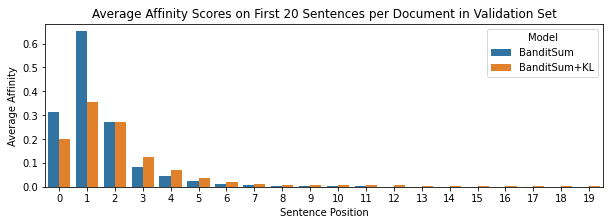
\includegraphics[width=0.9\linewidth]{fig/avg_affs.png}
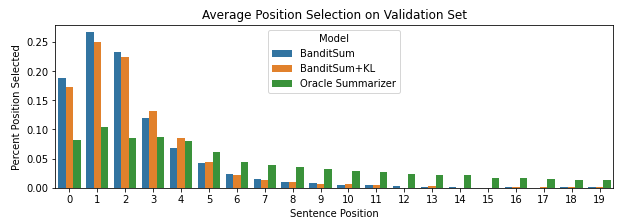
\includegraphics[width=0.9\linewidth]{fig/pos_avg.png}
\caption[Average affinity scores and average position selected for the BanditSum and BanditSum+KL models.]{(Top) Average affinity scores for the BanditSum and BanditSum+KL models. Note that the original model has far higher affinity on average for the first two sentence positions, while our proposed model has a more even distribution. (Bottom) Average position selected for the same models. We observe similar trends as the affinity score distribution, though the BanditSum+KL method remains far from the oracle positions.}
\label{fig:avg_pos}
\end{figure}

\begin{figure}[h]
    \centering
    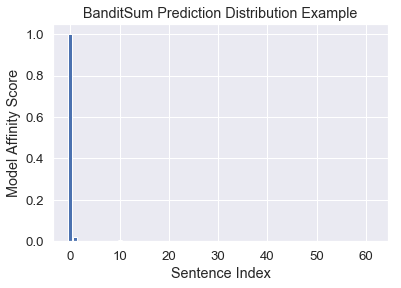
\includegraphics[width=0.48\textwidth]{fig/banditsum_pred_dist.png}
    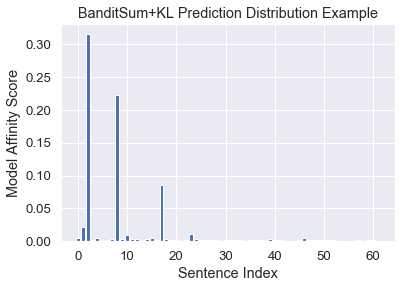
\includegraphics[width=0.48\textwidth]{fig/mixed_rouge_pred_dist.png}
    \caption[Example of the BanditSum vs. BanditSum+KL prediction distributions.]{Example of the BanditSum prediction distribution (left) vs. the BanditSum+KL prediction distribution (right) on the same given article from the validation set. The original formulation is more prone to lead bias compared to our proposed method, as demonstrated here.}
    \label{fig:pred_dist}
\end{figure}

%%%%%%%%%%%%%%%%%%%%%%%%%%%%%%%%%%%%%%%%%%%%%%%%%%%%%
% Lead Classification
%%%%%%%%%%%%%%%%%%%%%%%%%%%%%%%%%%%%%%%%%%%%%%%%%%%%%
\chapter{Summarizing by Classifying Lead Performance}
Chapter 4's results suggest that methods addressing model dependence on positional cues can be an effective way to boost summarization performance. The previous chapter's auxiliary loss method is able to decrease how frequently the base model selects from leading sentences, while also significantly improving summary quality. Although the auxiliary loss method's summarization improvement is statistically significant, it does not offer extraordinary gains over baselines. Figure \ref{fig:avg_pos} reveals that the method only offers modest reductions in how often lead sentences are selected and does not approach the percentage an oracle summarizer selects from the lead.

The results do not necessarily suggest that addressing positional biases is an ineffective strategy. Previous works such as \cite{kedzie2018content} and our own experiments in Chapter 3 have already shown that positional cues represent a major bottleneck for learning summarization. Instead, we suspect that the auxiliary loss methods are not sufficiently aggressive enough to counter the effects of lead bias. For these reasons, we would prefer a model formulation that integrates the ideas of lead bias more centrally.

We hypothesize that articles with a strong lead (i.e. the lead forms an accurate summary) are fundamentally different from cases with a weak lead, such that a classifier could distinguish between these two cases. We look to build such a classifier, so that we can apply different summarization strategies for the two scenarios. In this chapter, we detail this new classification task, the model formulation, the challenges surrounding the task and the resulting model's summarization capabilities.

\section{Classification Task}
We first define how to categorize articles based on the lead baseline's strength. Since there is a large variance between the highest achievable ROUGE score between different articles, we avoid categorizing articles solely based on the lead ROUGE score. For example, if the lead baseline achieves 30.0 ROUGE-1 on both articles $A$ and $B$, but the oracle summarizer respectively achieves 60.0 and 30.0 ROUGE-1, we should avoid placing $A$ and $B$ in the same category. To avoid this scenario, we rank articles by how well the lead performs in relation to an oracle summarizer:

\begin{equation}
\mathrm{Proportion\ Score}(D) = \frac{r_{lead}(D)}{r_{oracle}(D)}
\end{equation}
where $r_{lead}$ denotes the lead-3's ROUGE-1, -2 and -L average score on $D$, and $r_{oracle}$ denotes the same quantity using an oracle summarizer.
As previously, the lead is defined as the first 3 sentences in the document, while the oracle is defined in the same way as in Chapter \ref{chap:aux_loss}.

We also need to define a threshold value $T$ in order to divide articles. To determine an acceptable threshold value, we experiment with varying threshold values on the CNN / Daily Mail development set. For each threshold value, we divide the articles based on whether their proportion score falls below or above the given threshold. Documents below the threshold are summarized by the BandiSum+KL model, while documents above the threshold are handled by the lead-3 baseline. The results are shown in Figure \ref{fig:prop_value_thresh}.

\begin{figure}[h]
    \centering
    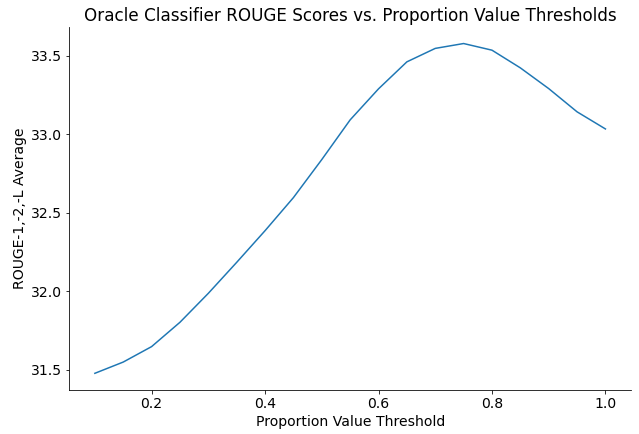
\includegraphics[width=0.75\linewidth]{fig/proportion_value_thresholds.png}
    \caption[ROUGE performance with varying proportion score thresholds.]{Each data point in this figure represents a trial with varying threshold $T$. In each trial, articles with proportion scores $<T$ are summarized by BanditSum+KL and otherwise summarized by the lead-3 baseline. The highest $\frac{1}{3}(R1+R2+RL)$ value is attained when $T = 0.75$.}
    \label{fig:prop_value_thresh}
\end{figure}

The highest gains in ROUGE performance are attained when the threshold $T = 0.75$, and we therefore use this value as the threshold in the following experiments.

Since distinguishing points very close to the threshold may be difficult for classifiers, we also experiment with removing articles close to the threshold $T$. After ranking all articles by their proportion score, we create subsets by removing articles close to the threshold. Specifically, we experiment with removing 20, 30, 50 and 60 percent from each of the training / development / testing data, centered around $T$. The subsets are named \Dtwenty, \Dthirty, \Dfifty{} and \Dsixty. We use \Dall{} to refer to the full dataset with no data removed. Furthermore, we designate the subset of articles with a proportion score less than $T$ as \Dlate, and greater than $T$ as \Dearly.

\section{Models}
In this section, we introduce the various components that comprise our summarization model. We describe (1) a strong baseline using BanditSum and BERT, (2) the neural classifier model, and (3) the \BanSumEarly{} and \BanSumLate{} models for the \Dearly{} and \Dlate{} subsets.

\subsection{Neural Classifier}
The centrepiece of our summarization approach is a classifier separating articles with a strong lead from articles where summary-worthy sentences appear later. We experiment with four model formulations. A common element of these models is they encode the leading three sentences separately from the overall document and recombine the embeddings to classify the article. The goal of this formulation is to allow the model to learn the interactions between the article's leading sentences and the overall document, in order to properly classify the article. The four models are as follows:
\begin{itemize}
    \item \textbf{Concatenation model:} After separately encoding the first three leading sentences and the entire document with BERT, we extract the [CLS] token embeddings as sentence representations. We then use separate LSTMs to run over the lead and document sentence embeddings, extracting the final hidden state of both. Shallow MLPs encode these representations to form a \textit{lead representation} $\mathbf{h}_L$ and a \textit{document representation} $\mathbf{h}_D$. Finally the lead and whole document representations are concatenated and a logistic layer assigns a probability of a high proportion score:
    \begin{equation}
        p\left(\frac{r_{lead}(D)}{r_{oracle}(D)} > T \ \middle\vert\  \mathbf{h}_L, \mathbf{h}_D \right) = \sigma \left(w_{out}\ [ \mathbf{h}_L ; \mathbf{h}_D ] \right)
    \end{equation}
    
    \item \textbf{Bilinear model:} This model is similar to the concatenation model but instead of concatenating the lead and document representations, a bilinear map combines the embeddings.
    \begin{equation}
        p\left(\frac{r_{lead}(D)}{r_{oracle}(D)} > T \ \middle\vert\  \mathbf{h}_L, \mathbf{h}_D \right) = \sigma \left( \mathbf{h}_L^T W_{out}\ \mathbf{h}_D \right)
    \end{equation}
    
    \item \textbf{Separate-BERT model:} This model follows the concatenation model but separate BERT encoders are used to produce the lead and document representations.
    \item \textbf{No-lead baseline:} The leading three sentences are not separately encoded. After BERT encodes the document, the first [CLS] token representation is provided as input to a logistic layer which maps this output to a probability between 0 and 1.
\end{itemize}

\subsection{\Dearly{} and \Dlate{} Subset Training}
After articles are classified, our approach requires two different summarization methods to handle each case. A reasonable strategy is to train separate summarization systems on the \Dearly{} and \Dlate{} subsets. We first define a base model based on BanditSum, then detail how to specialize the model on the two cases through subset training.

\subsubsection{Base Model: BanditSum+BERT}
% Describe the new model architecture and the table below
We continue to use BanditSum in these experiments, though we replace the sentence encoder from the original formulation with BERT \parencite{bert}. Given a document $D$ with sentences $s_1,\dots,s_N$, we encode it using BERT and use the [CLS] token as a sentence embedding, similar to the BertSum summarization model \parencite{bertsum}. These sentence embeddings are then fed to a multi-layer perceptron decoder in order to produce a \textit{sentence affinity} $\pi_i \in [0, 1]$ for each sentence $s_i \in D$. Essentially, we compute:

\begin{align}
    \pi_i &= \mathrm{MLP}(h_i) \\
    h_1,\dots,h_N &= \mathrm{BERT}(D)
\end{align}

The MLP structure follows BanditSum's decoder specifications and the remaining model details such as the reinforcement learning-based objective function follow BanditSum's details as well \parencite{dong2018banditsum}.

\subsubsection{Training on Data Subsets}
In order to specialize the base model towards summarizing \Dearly{} and \Dlate{} articles, we train two separate versions of BanditSum+BERT, restricted to the \Dearly{} and \Dlate{} subsets. Our hypothesis is that articles where the lead baseline performs well require a different summarization strategy than cases where the lead is weak. We use \BanSumEarly{} to denote the model trained on \Dearly{} and likewise, use \BanSumLate{} for the model trained on \Dlate{}.

\subsection{Summarization through Classification: LeadClassifySum}
The final summarization model is a straightforward pipeline of the previous components. Given an article, the classifier predicts if it belongs in \Dearly{} or \Dlate{}, and the appropriate model is then used to summarize it. After finding that \BanSumEarly{} solely learns positional cues and chooses indices nearly always matching the lead-3 baseline, we instead use the simpler lead-3 baseline to summarize cases in \Dearly{}. We use \BanSumLate{} to summarize articles in \Dlate{}. This final model is named LeadClassifySum.

\section{Experiments}
% Classifier
For each of the \Dtwenty{}, \Dthirty{}, \Dfifty{} and \Dsixty{} subsets, we train the four classification models to separate articles with a proportion score less than $T$ from ones greater than $T$. We also experiment with a setting where no articles are removed, i.e. using \Dall{}. Every model is trained to reduce the cross-entropy loss between its prediction and the gold label. For each training subset, we test the model using a subset of the test set that respects the same threshold boundaries as the training subset. We implement data re-weighting to reduce the effects of class imbalance, and we employ gradient clipping with a maximum gradient norm of 1.0.

% Base model
We train the BanditSum+BERT model on the CNN / Daily Mail dataset, converging after 6 epochs. For both \Dearly{} and \Dlate{} subsets, we train separate BanditSum+BERT models, with the late version converging within 10 epochs and the early version within 5 epochs.

For all experiments, we employ the Hugging Face `bert-base-uncased' BERT implementation to build our models \parencite{Wolf2019HuggingFacesTS}. We use Adam to optimize model parameters, with PyTorch's default momentum configuration \parencite{adam_kingma2014adam, pytorch}. We tune the learning rate for each of these experiments using the Tune library \parencite{tune}.

\section{Results}
\subsection{Classification Results}
Results across all model variations are very similar for at least one learning rate configuration. The results for the Bilinear model are shown in Table \ref{tab:class_acc}. All subsets experience a striking degree of overfitting, with each subset resulting in greater than 20\% difference between the training and testing accuracy. In Table \ref{tab:maj_base_comp}, we compare the Bilinear model to a simple majority baseline. Apart from the \Dall{} setting, the classifier outperforms the majority baseline, suggesting that the classifier learns non-trivial cues from the training data. There is also a notable increase in test set accuracy as the amount of data removed increases, with an 11\% increase between the \Dall{} and \Dsixty{} dataset. However, overall, overfitting prevents our classifier implementations from being practical.

\begin{table}[h]
    \centering
    \begin{tabular}{c|c|c}
    \toprule
    Dataset	&	Training Accuracy (\%)	&	Test Accuracy (\%)	\\ \hline
    \Dall	&	81.64	&	62.5	\\
    \Dtwenty	&	90.29	&	65.09	\\
    \Dthirty	&	95.74	&	67.09	\\
    \Dfifty	&	93.31	&	71.9	\\
    \Dsixty	&	93.61	&	73.49	\\ \bottomrule
    \end{tabular}
    \caption[Classification results for the Bilinear model on various data subsets.]{Classification results for the Bilinear model on various data subsets. We notice greater test accuracy as the amount of data removed increases; however, strong overfitting prevents the classifiers from being practical for our purposes.}
    \label{tab:class_acc}
\end{table}

\begin{table}[h]
    \centering
    \begin{tabular}{c|c|c|c|c|c}
    \toprule
    Model	&	\multicolumn{5}{c}{Accuracy (\%)}		\\	
    &	\Dall{}	&	\Dtwenty{}	&	\Dthirty{}	&	\Dfifty{}	&	\Dsixty{}	\\ \hline
    Majority Baseline	&	64.62	&	52.61	&	52.94	&	53.29	&	53.16	\\
    Bilinear Model	&	62.5	&	65.09	&	67.09	&	71.9	&	73.49	\\ \bottomrule
    \end{tabular}
    \caption[Classification accuracy comparison for the bilinear model against a majority baseline.]{Apart from the \Dall{} dataset, the Bilinear model is able to outperform a majority baseline on the classification task.}
    \label{tab:maj_base_comp}
\end{table}

\subsection{\Dearly{} and \Dlate{} Results}
% D_late results
The results for \Dlate{} and \Dearly{} are displayed in Tables \ref{tab:late_subset} and \ref{tab:early_subset} respectively. On \Dlate{}, subset training benefits the BanditSum+BERT model considerably, as we see large jumps in ROUGE-1, -2 and -L metrics. There is also a strong decrease in the lead overlap, as the \BanSumLate{} model is exposed to less positional bias compared to the baseline model. These results confirm that separating articles with weak lead performance is important for summarization, and that subset training can help models focus on a specific strategy for the \Dlate{} subset.

% D_early results
The \Dearly{} experiment shows even greater gains in ROUGE performance, around 2 points across all three ROUGE metrics. However, in this case, positional biases clearly play a dominating role in the model's learning process, as the model exactly copies the lead-3 baseline and achieves the same performance. Unfortunately, the model fails to pick up on deeper cues and its ROUGE scores remain far from the oracle's.

\begin{table}[t]
    \centering
    \begin{tabular}{c|c|c|c|c}
    \toprule
    Model	&	ROUGE-1	&	ROUGE-2	&	ROUGE-L	&	Lead Overlap (\%)	\\ \hline
    BanditSum+BERT	&	40.17	&	17.56	&	36.61	&	53.20	\\ 
    \BanSumLate	&	40.75	&	18.17	&	37.30	&	33.37	\\ \hline
    Lead-3	&	35.32	&	13.38	&	31.77	&	100.0	\\ 
    Oracle	&	57.19	&	33.50	&	53.94	&	17.13	\\
    \bottomrule
    \end{tabular}
    \caption[ROUGE results on \Dlate{}.]{Results on CNN / Daily Mail test articles with proportion score less than $T = 0.75$, corresponding to training on \Dlate. The \BanSumLate{} model noticeably outperforms BanditSum+BERT and selects the leading sentences less often.}
    \label{tab:late_subset}
\end{table}

\begin{table}[t]
    \centering
    \begin{tabular}{c|c|c|c|c}
    \toprule
    Model &	ROUGE-1	&	ROUGE-2	&	ROUGE-L	&	Lead Overlap (\%)	\\ \hline
    BanditSum+BERT	&	47.01	&	22.84	&	43.18	&	67.50	\\
    \BanSumEarly	&	49.01	&	24.52	&	45.04	&	99.99	\\ \hline
    Lead-3	&	49.01	&	24.52	&	45.04	&	100.0	\\
    Oracle	&	56.16	&	30.70	&	52.45	&	45.70	\\ \bottomrule
    \end{tabular}
    \caption[ROUGE results on \Dearly{}.]{Results on CNN / Daily Mail test articles with proportion score less than $T = 0.75$, corresponding to training on \Dearly. Although \BanSumEarly{} outperforms BanditSum+BERT significantly, positional cues dominate the learning signal for \BanSumEarly{}. In the end, it is indistinguishable from the lead-3 baseline.}
    \label{tab:early_subset}
\end{table}

\subsection{Summarization Results}
The main summarization results on the CNN / Daily Mail test set are shown in Table \ref{tab:banditsum_bert}. 

\subsubsection{BanditSum+BERT Baseline}
The BanditSum+BERT markedly outperforms BanditSum across all three ROUGE metrics, indicating that BERT's encodings are far more suitable for this summarization task than LSTMs. Besides a noticeable increase in ROUGE, the model also selects significantly less from the lead than both BanditSum and the BanditSum+KL model. One possible explanation is that BERT acts as a regularizer for sentence position, and its strong language modelling abilities help it from being distracted by position cues.

\subsubsection{LeadClassifySum}
Hampered by a weak classifier, the LeadClassifySum approach is unable to surpass its baseline in terms of ROUGE. Curiously, the degree of lead overlap actually increases, further reflecting on the classifier's inability to properly separate strong-lead articles from weak ones. The summarization approach hinges on a capable classifier, and in the absence of one, this result is expected.

\begin{table}[h]
    \centering
    \begin{tabular}{c|c|c|c|c}
    \toprule
    Model	&	ROUGE-1	&	ROUGE-2	&	ROUGE-L	&	Lead Overlap (\%)	\\ \hline
    Lead-3	&	40.06	&	17.53	&	36.18	&	100.0	\\
    BanditSum 	&	41.68	&	18.78	&	38.00	&	69.87	\\
    BanditSum+BERT	&	42.70	&	19.40	&	39.03	&	57.52	\\ \hline
    LeadClassifySum	&	41.82	&	18.62	&	38.12	&	73.52	\\ \hline
    Oracle Classifier	&	43.73	&	20.49	&	40.13	&	52.02	\\
    Oracle	&	56.53	&	32.65	&	53.12	&	27.24	\\ \bottomrule
    \end{tabular}
    \caption[LeadClassifySum ROUGE results on CNN / Daily Mail test set.]{Results from various models on the CNN / Daily Mail test set. While BanditSum+BERT outperforms BanditSum, both are surpassed by the Oracle Classifier and true Oracle scores.}
    \label{tab:banditsum_bert}
\end{table}

\section{Analysis}
\subsection{Exploring Threshold Values}
\begin{figure}[h]
    \centering
    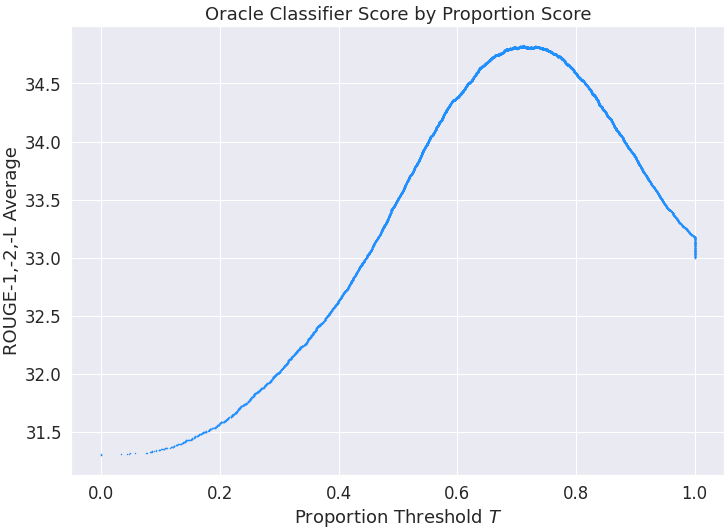
\includegraphics[width=0.75\linewidth]{fig/oracle_lead_classifier_thresholds.png}
    \caption[A fine-grained analysis of summarization performance change when the threshold is varied.]{By running both \BanSumLate{} and Lead-3 models over the entire test set, we can visualize how the ROUGE-1, -2 and -L average score changes on an article-by-article basis when varying the threshold $T$. This experiment validates our choice of $T$ and shows that only a single optimum exists.}
    \label{fig:oracle_classifier_threshold}
\end{figure}

A natural question to ask is what an upper performance bound would be from using this approach. To this end, we run an oracle classifier over the CNN / Daily Mail test set to correctly label articles with their proportion score. Articles with a proportion score less than $T$ are then summarized with the \BanSumLate{} model. Conversely, articles with a proportion score greater than $T$ are summarized by the lead-3 baseline.

The Oracle Classifier results are displayed in Table \ref{tab:banditsum_bert}. The noticeable performance gain of over 1 point in ROUGE-1, -2 and -L metrics suggest that our lead classifier approach is a viable approach to summarization. This oracle method is furthermore able to decrease lead overlap by 5.5\% compared to the base \BanSumLate{} model, achieving a closer degree of lead overlap as the true oracle model.

We also want to further validate our choice of $T$. The experiment shown in Fig. \ref{fig:prop_value_thresh} gives an adequate estimate of a good threshold value. However, we would prefer to use stronger baselines as the base models and analyze the results on a fine-grained article-by-article basis.

We first create summaries for the whole CNN / Daily Mail test set with both lead-3 and \BanSumLate{} models, and sort all articles by their proportion scores. We then sweep through the sorted test set, marking the change in overall average ROUGE-1, -2 and -L scores as $T$ varies. The results are shown in Figure \ref{fig:oracle_classifier_threshold}. The peak ROUGE score, occurring at $T=0.71$, shows the possible gains over the \BanSumLate{} model (far right point) and lead-3 model (far left point). Figure \ref{fig:oracle_classifier_threshold} also demonstrates that only a single optimal threshold value exists, and that our choice of $T$ is justified.

\subsection{Classifier Regularization}
In an effort to reduce the degree of overfitting, we explore a variety of regularization techniques to reduce the gap between the training and testing accuracies. We experiment with the following techniques:
\begin{itemize}
    \item \textbf{Weight decay} is a common technique for regularizing parameters which involves multiplying each weight by a factor slightly less than one after each step. We explore a variety of weight decay terms to regularize model parameters.
    \item \textbf{Reducing model complexity:} We halve both the LSTM decoders' hidden size and the logistic classifier size to explore if reducing model size improves generalization.
    \item \textbf{PCA on BERT outputs:} BERT's output representations are 768-dimensional vectors, which may be too large for the task. Using a version of BERT with lower-dimensional outputs requires re-training the entire BERT model from scratch, which is computationally infeasible. Instead, after fine-tuning BERT on the classification task, we fix BERT's parameters and employ PCA to reduce the output dimension to 300. We then continue fine-tuning the decoders using the lower-dimensional outputs.
    \item \textbf{Freeze BERT outputs:} In order to reduce the number of trainable parameters, we fix BERT's parameters, and only fine-tune the remaining weights.
\end{itemize}
We do not explore using dropout as the BERT encoder already employs it.

Unfortunately, none of the above regularization techniques significantly changes classification accuracy on the test set. Freezing BERT outputs decreases accuracy by around 8\%. Further regularization techniques may be beneficial to the task, but ultimately the solution may require alternate model formulations to overcome the gaps in accuracy.

\vspace{-4px}
\section{Conclusion}
In this chapter, we conjecture that separating articles with strong or weak leads can aid automatic summarization. To partition the dataset, we define a document's \textit{Proportion Score}, the ratio of the lead to oracle ROUGE score. We run experiments using the lead-3 baseline and the BanditSum+KL model to determine an effective threshold $T$ to partition the CNN / Daily Mail dataset.

We design classifiers to divide documents by their proportion score. Despite regularization attempts, overfitting remains a bottleneck for our approach. Future methods may require alternate model formulations or stronger regularization techniques.

We proceed to build a base model using BanditSum with a BERT encoder, and show that this model outperforms the original BanditSum summarizer. After partitioning the training dataset based on proportion score, we train separate summarizers on the subsets. On the late subset, where the documents' proportion scores are less than $T$, \BanSumLate{} is able to create better summaries, presumably because its representations are less biased towards positional cues. In contrast, \BanSumEarly{} summarization performance increases on the early subset, but the model exclusively learns to copy the lead baseline.

Using an oracle classifier, we show that the summarization performance can improve up to 1 point across all ROUGE-1, -2 and -L metrics. We examine how performance gains change on an article-by-article basis, showing that only a single optimum occurs at $T = 0.71$.


%%%%%%%%%%%%%%%%%%%%%%%%%%%%%%%%%%%%%%%%%%%%%%%%%%%%%
% Conclusion
%%%%%%%%%%%%%%%%%%%%%%%%%%%%%%%%%%%%%%%%%%%%%%%%%%%%%
\chapter{Conclusion}
In this work, we have investigated summarization systems and how positional biases affect these systems' learning process. Motivated by \cite{kedzie2018content}'s work and our own experiments showing that current summarization systems are heavily affected by positional cues, we design novel methods to counter the dominance of these signals.

Our first method involves augmenting an existing gradient descent-based summarization model with an auxiliary loss objective. For a given input article, this loss objective estimates each sentence's value by computing the sentence-level ROUGE score compared to the reference summary. It then encourages the model to match these sentence-value estimates using the KL divergence between the model's predictions and the estimates. We test this method with a state-of-the-art summarization system, BanditSum \parencite{dong2018banditsum}, and find that our method can significantly improve summary quality. 

Although the improvements are noteworthy, the resulting model is still hampered by an overreliance on lead bias. Evidence for this lingering issue is seen in Figure \ref{fig:avg_pos}, as the oracle summarizer extracts leading sentences far less than the BanditSum+KL method. Some extensions to this method could include other algorithms to combine the loss functions such as MAML \parencite{maml}, or investigating RL methods aimed at promoting exploration such as the Soft-Actor Critic algorithm \parencite{sac}.

After hypothesizing that articles with a strong vs. weak lead require different summarization strategies, we design a second novel summarization method based around classifying whether an article's lead contains summary-worthy sentences. We find that by partitioning the training dataset and training separate summarization systems on these subsets, we can achieve greater performance on both subsets. We note that in the case of the \Dearly{} subset, the model's learning is dominated by positional bias, and it learns to mimic the lead-3 baseline exactly. Training a classifier proves to be a much more difficult task, especially with regards to overfitting.

% Limitations
Assuming an accurate classifier is achievable, future summarization approaches may render this approach redundant. Emerging summarization models, such as BertSum and BART \parencite{bertsum, lewis2019bart}, have taken advantage of large unsupervised language model pre-training in their approaches. In particular, the authors of BertSum show that their method is able extract sentences further in the document compared to a competitive baseline, and that the extracted indices are more similar to an oracle summarizer. Compared to previous models such as BanditSum, BertSum is more robust with respect to lead bias effects, despite having no explicit target objective aimed at countering this damaging signal. This may mean that explicit lead bias regularization is not necessary, as long as the model can sufficiently balance positional cues with semantic ones.

% Conclude: lead bias is an important factor for summarization
Regardless of how future summarization models operate, we have shown that positional biases are an important consideration when designing summarization systems. Creating models that understand how to properly balance positional cues and value sentences correctly represents a major milestone towards truly practical summarization systems.


%%%%%%%%%%%%%%%%%%%%%%%%%%%%%%%%%%%%%%%%%%%%%%%%%%%%%
% Bibliography
%%%%%%%%%%%%%%%%%%%%%%%%%%%%%%%%%%%%%%%%%%%%%%%%%%%%%
%\bibliography{library}
%\bibliographystyle{plain}
\printbibliography
\end{document}